\documentclass[a4paper,12pt]{report}
\usepackage[T2A]{fontenc}
\usepackage[utf8]{inputenc}
\usepackage[english,russian]{babel}
\usepackage{graphicx}
\usepackage{wrapfig}
\usepackage{mathtext} 				% русские буквы в фомулах
\usepackage{amsmath,amsfonts,amssymb,amsthm,mathtools} % AMS
\usepackage{icomma} % "Умная" запятая: $0,2$ --- число, $0, 2$ --- перечисление
\usepackage{capt-of}
\usepackage{appendix}
\usepackage{multirow}
\usepackage{hyperref}
\usepackage{floatrow}
\usepackage[left=2cm,right=2cm,
    top=2cm,bottom=2cm,bindingoffset=0cm]{geometry}
\usepackage{multicol} % Несколько колонок
\usepackage{gensymb}
\title{Отчёт по лабораторной работе №6.9.1

Закон Кюри-Вейса и обменное взаимодействие в ферромагнетиках}
\author{Плюскова Н.А. Б04-004 }
\date{\today}

\begin{document}

\maketitle

\section*{1. Аннотация}
В данной работе исследуется температурная зависимость магнитной восприимчивости ферромагнетика в парамагнитной области - выше точки Кюри. По полученной в работе температуре Кюри оценивается энергия обменного взаимодействия. Объектом исследования является металлический гадолиний.


\section*{2. Теоретическое введение}
\subsection*{2.1 Феноменологическое описание ферромагнетиков: парамагнитная фаза и эффективное поле Вейсса}

Намагниченностью называется магнитный момент $І$ единицы объёма, который связан с внешним магнитным полем $H$ через магнитную восприимчивость $\varkappa$: $I = \varkappa H$

Рассмотрим восприимчивость парамагнитного вещества, в котором магнитный момент атома обусловлен только спином одного электрона. Тогда в магнитном поле у атома возникают два возможных уровня энергии: $E_{-}=-\mu B$ и $E_{+}=+\mu B$, причем в низкоэнергетичном состоянии $Е_-$ магнитный момент параллелен магнитному полю.

В соответствии с Больцмановским распределением отношение числа электронов $N_{+}$ с энергией $E_{+}$ к числу электронов $N_-$ с энергией $E_-$ равно

\begin{equation}\label{bolzman}
    \frac{N_{+}}{N_{-}}=\exp \left(-\frac{2 \mu B}{k_{\mathrm{B}} T}\right) \simeq 1-\frac{2 \mu B}{k_{\mathrm{B}} T}
\end{equation}

Намагниченность вещества определяется только разностью чисел электронов,
магнитные моменты которых ориентированы по полю или против поля, а поскольку мы рассматриваем проекцию магнитного момента на одну ось, то парамагнитная часть восприимчивости равна:

\begin{equation}\label{kappa-easy}
    \varkappa = \frac{I}{H} = N \frac{\mu^2}{k_B T} = N \frac{g^{2} \mu_{\mathrm{B}}^{2} S(S+1)}{3 k_{\mathrm{B}} T}
\end{equation}

Для описания взаимодействия соседних электронов в ферромагнетике предположим, что в ферромагнетике имеется некоторое эффективное магнитное поле $H_{\text {эфф}}$. Величина обменного поля пропорциональна имеющейся намагниченности образца: $H_{\text{эфф}} = \lambda I$, где $\lambda$ -- некоторая константа. Тогда, учитывая поправку на дополнительное поле $H_{\text{эфф}}$, получим закон Кюри-Вейсса:

\begin{equation}\label{C-W}
    \varkappa=\frac{I}{H}=N \frac{g^{2} \mu_{\mathrm{B}}^{2} S(S+1)}{3 k_{\mathrm{B}}(T-\Theta)} \propto \frac{1}{T-\Theta}
\end{equation}

Где $\Theta=\frac{N \mu^{2} \lambda}{k_{\mathrm{B}}}=N \frac{g^{2} \mu_{\mathrm{B}}^{2} S(S+1)}{3 k_{\mathrm{B}}} \lambda$ -- параметр, имеющий размерность температуры.

Этот закон носит приближенный характер и не позволяет описать, что происходит в ферромагнитой области, но достаточно точно характеризует температурную зависимость магнитной восприимчивости в парамагнитной фазе. 

\subsection*{2.2 Связь эффективного поля Вейсса с обменным интегралом.}

Энергия обменного взаимодейтвия $U_\text{обм}$ атомов $i$ и $j$ представляет собой разность между средними значениями кулоновской энергии для параллельных и антипараллельных спинов $S_i$ и $S_j$, а $Ј$ -- коэффициент пропорциональности, называемый обменным интегралом, величина которого зависит от степени перекрытия распределённых зарядов атомов $i$ и $ј$.

\begin{equation}\label{energy}
    U_\text{обм} = -2 J S_i S_j
\end{equation}

Установим приближенно связь между обменным интегралом $Ј$ и константой Вейсса $\lambda$. Найдем энергию $U_\text{пер}$, требуемую для переворота данного спина в присутствии всех других спинов его ближайших соседей. С одной стороны, эта энергия вдвое больше обменной энергии системы с какой-то определенной ориентацией спина. С другой стороны, каждый магнитный атом испытывает действие эффективного поля, следовательно, воздействиевсех спинов на данный характеризуется средней намагниченностью $І=\mu/V$, и мы можем записать равенство

$$2\cdot2Jn S^2 = U_{\text{пep}}=2 \mu H_{\text{эфф}} =2 \mu \frac{\lambda \mu}{V}$$

Выразив константу $\lambda$ из температуры $\Theta$, мы получаем:

\begin{equation}\label{obm-int}
    J=\frac{3 k_{\text {B }} \Theta}{2 n S(S+1)}
\end{equation}

\section*{3. Экспериментальная установка и принцип измерений}

\begin{figure}[h!]
\begin{center}
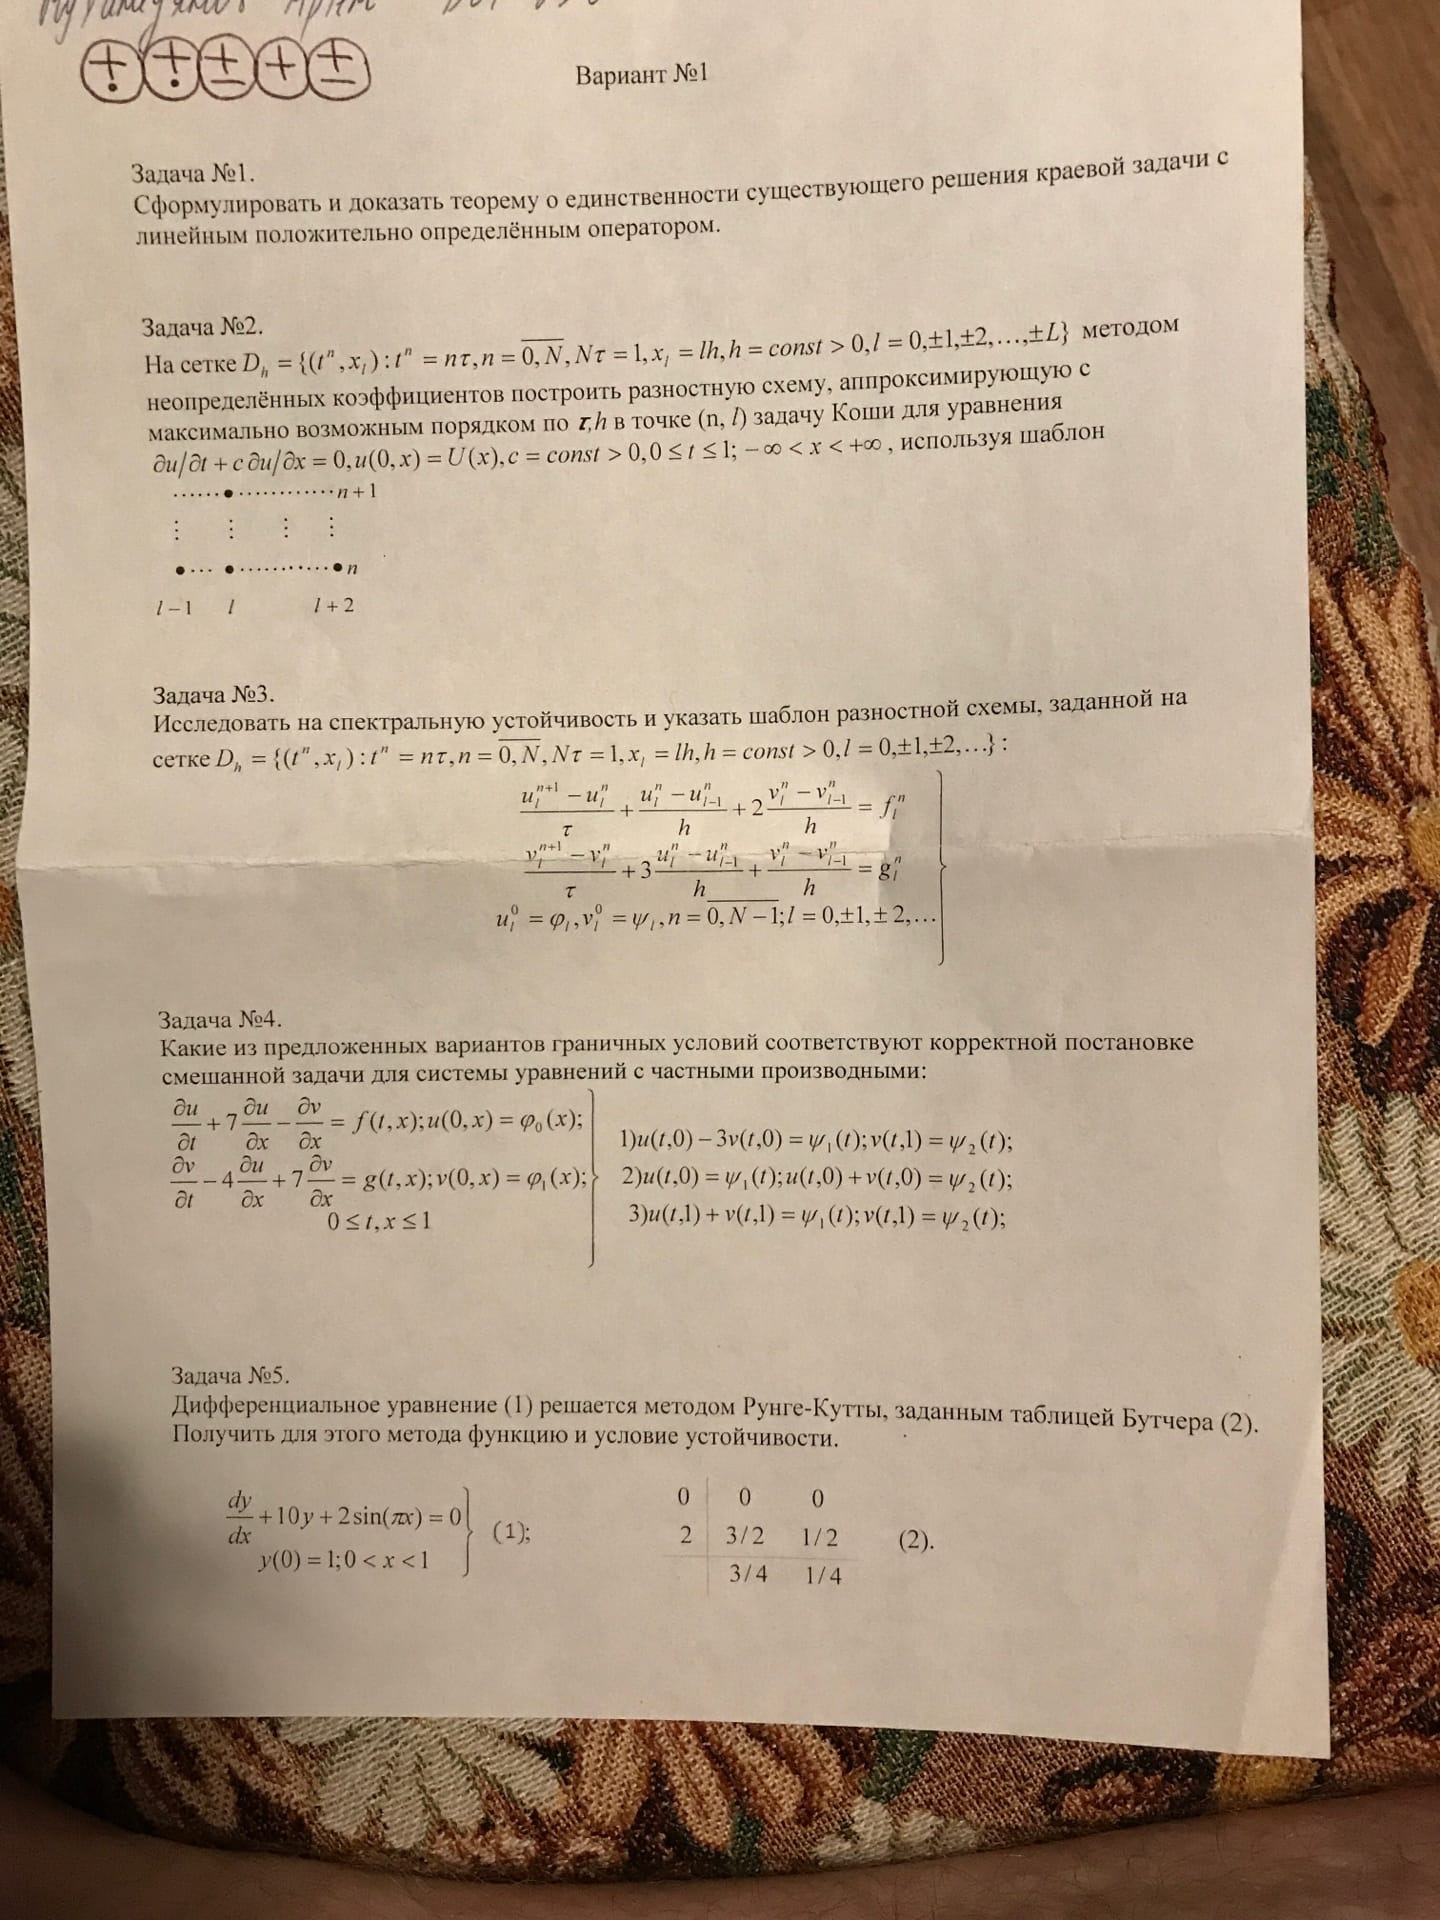
\includegraphics[scale=0.5]{1.jpg}
\caption{Схема экспериментальной установки}
\end{center}
\end{figure}

Экспериментальная установка для измерения восприимчивости магнетиков приведена на рис. 1.  Ферромагнитный образец 1 располагается внутри пустотелой катушки 2, которая является индуктивностью колебательного контура, входящего в состав LC-генератора. Частота колебаний генератора высвечивается на цифровом табло блока. Катушка самоиндукции помещена в термостат, представляющий собой массивный медный цилиндр 3, расположенный в пенопластовом корпусе 4. Образец помещен в тефлоновую капсулу. С помощью штока 5 капсулу можно перемещать вдоль оси катушки самоиндукции. Когда шток опущен, образец введен в катушку, а когда поднят -- образец из неё вынут.

Магнитная восприимчивость образца определяется по изменению самоиндукции, происходящему при его введении в катушку. Обозначая через $L$ индуктивность катушки с образцом и через $L_0$ её индуктивность в отсутствии образца, получим:

$$ \frac{L-L_{0}}{L_{0}}=\frac{\Delta L}{L_{0}}=\mu-1 = 4 \pi \varkappa$$

Учитывая, что частота $f$ колебательного LС-контура определяется выражением $\frac{1}{f}=2 \pi \sqrt{L C},$ получим:

\begin{equation}\label{dependency}
    \frac{1}{\varkappa} \propto \frac{f^{2}}{f_{0}^{2}-f^{2}}
\end{equation}  
	


\section*{4. Результаты эксперимента и обработка данных}
При выполнении работы образец сначала охлаждается ниже точки Кюри, а затем медленно нагревается. Исследуем зависимость частот $f$ и $f_0$ от температуры, постепенно нагревая образец. Измерения  проводим в интервале от $2~^\circ \text{C}$ до $50~^\circ \text{C}$ с шагом в примерно $3~^\circ \text{C}$, результаты представлены в Таблице 1 в разделе Приложение.

Результаты измерения изобразим на графике (Рис. 2) в координатах $\left( T, \frac{f^2}{f_0^2-f^2}\right)$.

\begin{figure}[H]
    \centering
    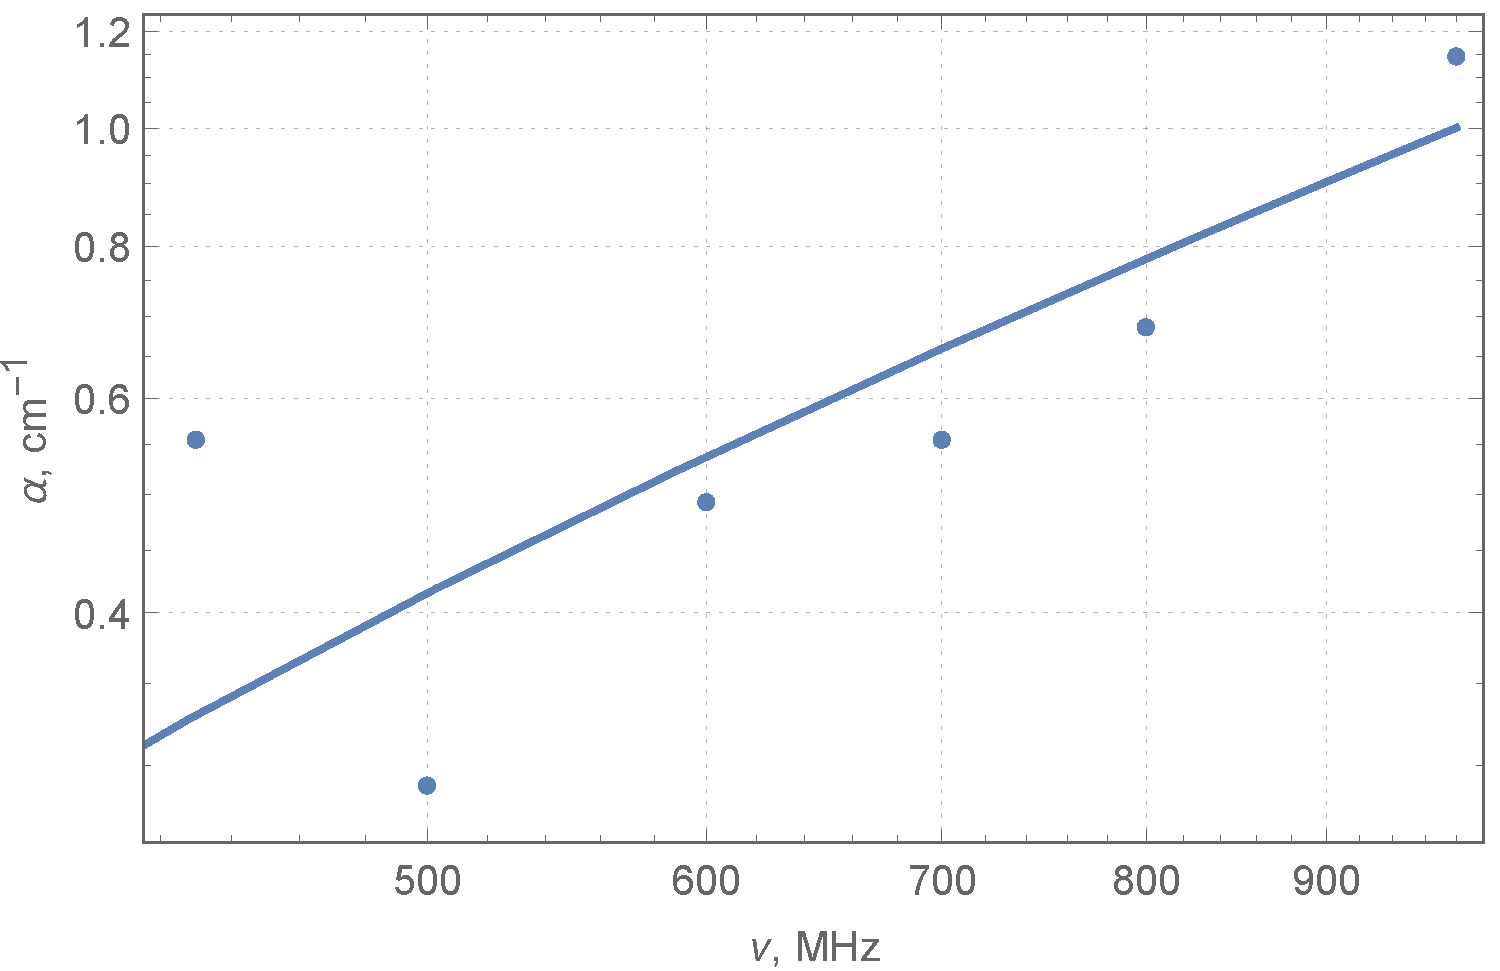
\includegraphics[width=0.7\linewidth]{graph}
    \caption{Зависимость $\cfrac{f^2}{f_0^2-f^2}(T)$}
\end{figure}

Линейный участок аппроксимируем прямой, искомые коэффициенты из метода наименьшних квадратов равны:

\[k = 8.78 \pm 0.40\]
\[b = -165.87 \pm 13.14\]

Пользуясь соотношениями \eqref{C-W} и \eqref{dependency}, получаем

\[\Theta = -\dfrac{b}{k} = 18.90 \pm 1.66~\text{$^\circ$C} = 291.9 \pm 25.6~\text{K}\]

Пользуясь формулой \eqref{obm-int}, оценим величину обменного интеграла, считая, что для гадолиния $n = 12$, $S = 7/2$:

\[J = 0.200\pm 0.019~\text{мэВ}\]


\section*{5. Вывод}
В ходе работы была исследована температурная зависимость магнитной восприимчивости гадолиния и определена температура Кюри $\Theta = 291.9 \pm 25.6~\text{К}$, что в пределах $\sigma$ совпадает с табличным значением $293.4~\text{К}$. По измеренным данным видно, что закон Кюри-Вейса не выполняется при температурах, ниже $\Theta$, т.е. в ферромагнитной области. По полученному значению $\Theta$ был оценен обменный интеграл $J = 0.200\pm 0.019~\text{мэВ}$.

Возможные причины расхождения теоретического и экспериментального значений температуры Кюри:
\begin{itemize}
    \item Точно не успевали снимать значения частот $f$ и $f_{0}$
    \item Не учитывалась погрешность константы термопары
    \item Чем выше была температура, тем точнее были измерения $f$ и $f_{0}$
    \item При выполнении эксперимента сталкивались с проблемой колебаний температуры на 3-4 единицы вниз
\end{itemize}


\section*{6. Приложение}
\begin{table}[H]
\begin{tabular}{|c|c|c|c|c|c|c|}
\hline
$U$, мкВ & $\sigma_{U}$, мкВ         & $T,~^\circ \text{C}$     & $f$, кГц & $\sigma_{f}$, кГц           & $f_{0}$, кГц & $\sigma_{f_{0}}$, кГц          \\ \hline
-900   & \multirow{23}{*}{10} & 2,02  & 909,23 & \multirow{23}{*}{0,01} & 956,13  & \multirow{23}{*}{0,01} \\ \cline{1-1} \cline{3-4} \cline{6-6}
-780   &                      & 4,95  & 909,32 &                        & 956,51  &                        \\ \cline{1-1} \cline{3-4} \cline{6-6}
-750   &                      & 5,68  & 909,63 &                        & 955,71  &                        \\ \cline{1-1} \cline{3-4} \cline{6-6}
-660   &                      & 7,88  & 909,83 &                        & 955,83  &                        \\ \cline{1-1} \cline{3-4} \cline{6-6}
-540   &                      & 10,80 & 909,92 &                        & 956,03  &                        \\ \cline{1-1} \cline{3-4} \cline{6-6}
-440   &                      & 13,24 & 909,70 &                        & 955,73  &                        \\ \cline{1-1} \cline{3-4} \cline{6-6}
-410   &                      & 13,98 & 910,21 &                        & 955,78  &                        \\ \cline{1-1} \cline{3-4} \cline{6-6}
-380   &                      & 14,71 & 910,51 &                        & 955,83  &                        \\ \cline{1-1} \cline{3-4} \cline{6-6}
-350   &                      & 15,44 & 911,65 &                        & 955,94  &                        \\ \cline{1-1} \cline{3-4} \cline{6-6}
-310   &                      & 16,41 & 912,90 &                        & 955,80  &                        \\ \cline{1-1} \cline{3-4} \cline{6-6}
-270   &                      & 17,39 & 915,09 &                        & 955,89  &                        \\ \cline{1-1} \cline{3-4} \cline{6-6}
-250   &                      & 17,88 & 916,83 &                        & 955,81  &                        \\ \cline{1-1} \cline{3-4} \cline{6-6}
-220   &                      & 18,61 & 918,34 &                        & 955,99  &                        \\ \cline{1-1} \cline{3-4} \cline{6-6}
-190   &                      & 19,34 & 922,57 &                        & 955,98  &                        \\ \cline{1-1} \cline{3-4} \cline{6-6}
-170   &                      & 19,83 & 925,47 &                        & 956,00  &                        \\ \cline{1-1} \cline{3-4} \cline{6-6}
-150   &                      & 20,32 & 928,62 &                        & 956,04  &                        \\ \cline{1-1} \cline{3-4} \cline{6-6}
-130   &                      & 20,80 & 930,62 &                        & 955,98  &                        \\ \cline{1-1} \cline{3-4} \cline{6-6}
-110   &                      & 21,29 & 933,84 &                        & 956,05  &                        \\ \cline{1-1} \cline{3-4} \cline{6-6}
-90    &                      & 21,78 & 936,34 &                        & 955,98  &                        \\ \cline{1-1} \cline{3-4} \cline{6-6}
-70    &                      & 22,27 & 938,78 &                        & 956,01  &                        \\ \cline{1-1} \cline{3-4} \cline{6-6}
-50    &                      & 22,76 & 940,37 &                        & 955,82  &                        \\ \cline{1-1} \cline{3-4} \cline{6-6}
-20    &                      & 23,49 & 942,53 &                        & 955,97  &                        \\ \cline{1-1} \cline{3-4} \cline{6-6}
0      &                      & 23,98 & 943,87 &                        & 955,94  &                        \\ \hline
30     & \multirow{23}{*}{10} & 24,71 & 945,11 & \multirow{23}{*}{0,01} & 955,99  & \multirow{23}{*}{0,01} \\ \cline{1-1} \cline{3-4} \cline{6-6}
50     &                      & 25,20 & 946,34 &                        & 955,80  &                        \\ \cline{1-1} \cline{3-4} \cline{6-6}
70     &                      & 25,68 & 947,37 &                        & 955,94  &                        \\ \cline{1-1} \cline{3-4} \cline{6-6}
90     &                      & 26,17 & 948,24 &                        & 955,98  &                        \\ \cline{1-1} \cline{3-4} \cline{6-6}
110    &                      & 26,66 & 948,91 &                        & 956,00  &                        \\ \cline{1-1} \cline{3-4} \cline{6-6}
160    &                      & 27,88 & 950,12 &                        & 955,91  &                        \\ \cline{1-1} \cline{3-4} \cline{6-6}
210    &                      & 29,10 & 950,97 &                        & 955,84  &                        \\ \cline{1-1} \cline{3-4} \cline{6-6}
260    &                      & 30,32 & 951,46 &                        & 956,02  &                        \\ \cline{1-1} \cline{3-4} \cline{6-6}
310    &                      & 31,54 & 951,91 &                        & 956,01  &                        \\ \cline{1-1} \cline{3-4} \cline{6-6}
360    &                      & 32,76 & 952,33 &                        & 956,01  &                        \\ \cline{1-1} \cline{3-4} \cline{6-6}
410    &                      & 33,98 & 952,64 &                        & 956,01  &                        \\ \cline{1-1} \cline{3-4} \cline{6-6}
460    &                      & 35,20 & 952,80 &                        & 955,99  &                        \\ \cline{1-1} \cline{3-4} \cline{6-6}
510    &                      & 36,41 & 953,04 &                        & 955,97  &                        \\ \cline{1-1} \cline{3-4} \cline{6-6}
560    &                      & 37,63 & 953,20 &                        & 955,90  &                        \\ \cline{1-1} \cline{3-4} \cline{6-6}
610    &                      & 38,85 & 953,41 &                        & 956,02  &                        \\ \cline{1-1} \cline{3-4} \cline{6-6}
660    &                      & 40,07 & 953,54 &                        & 956,03  &                        \\ \cline{1-1} \cline{3-4} \cline{6-6}
710    &                      & 41,29 & 953,54 &                        & 956,03  &                        \\ \cline{1-1} \cline{3-4} \cline{6-6}
760    &                      & 42,51 & 953,75 &                        & 956,02  &                        \\ \cline{1-1} \cline{3-4} \cline{6-6}
810    &                      & 43,73 & 953,82 &                        & 955,98  &                        \\ \cline{1-1} \cline{3-4} \cline{6-6}
860    &                      & 44,95 & 953,94 &                        & 956,02  &                        \\ \cline{1-1} \cline{3-4} \cline{6-6}
910    &                      & 46,17 & 953,94 &                        & 955,97  &                        \\ \cline{1-1} \cline{3-4} \cline{6-6}
960    &                      & 47,39 & 954,03 &                        & 956,09  &                        \\ \cline{1-1} \cline{3-4} \cline{6-6}
990    &                      & 48,12 & 954,14 &                        & 956,08  &                        \\ \hline
\end{tabular}
\caption{Результаты измерений.}
\end{table} 
\end{document}
